\documentclass[a4paper,12pt]{scrbook} % preambuła
\usepackage[polish]{babel}
\usepackage[utf8]{inputenc} % utf8, cp1250
\usepackage{pslatex}
\usepackage[T1]{fontenc}
\usepackage{times}
\usepackage{geometry}
\usepackage{algorithm}
\usepackage{graphicx}
\usepackage{xcolor}
\usepackage{wrapfig}
\usepackage{amsmath}
\usepackage{subcaption}
\usepackage{algpseudocode}
\usepackage{pgfplots}
\newgeometry{tmargin=1.5cm, bmargin=1.5cm, lmargin=1.5cm, rmargin=1.5cm}

\begin{document}
\section{Prawo odbicia}
Promień padający, promień odbity i normalna do powierzchni granicznej wystawiona w punkcie padania promienia leżą w jednej płaszczyźnie i kąt padania równa się kątowi odbicia $\alpha _{1} = \alpha _{2}$. \\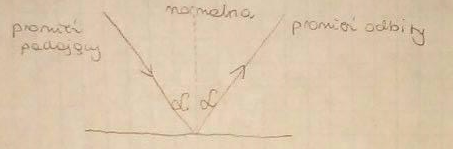
\includegraphics{prawo_odbicia}
W wyniku odbicia zmienia się tylko kierunek rozchodzenia się fali, nie zmienia się jej długość. 

\section{Załamanie światła na granicy dwóch ośrodków przeźroczystych}
Jeśli światło pada na granicę dwóch przeźroczystych ośrodków, to zwykle jego część odbija się(zgodnie z prawem odbicia),a część wchodzi do drugiego ośrodka, zmieniając na ogół kierunek swojego biegu. Mówimy wtedy, że światło się załamuje.

Prawo załamania (Prawo Snelliusa) sformułowane w 1621. Stosunek sinusa kąta padania do sinusa kąta załamania jest równy stosunkowi bezwzględnego współczynnika załamania ośrodka drugiego $n_{2}$ do bezwzględnego współczynnika załamania ośrodka pierwszego $n_{1}$, czyli współczynnikowi względnemu załamania światła ośrodka drugiego względem pierwszego.
\\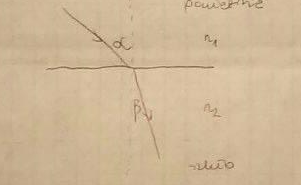
\includegraphics{prawo_zalamania}
\begin{equation}{\frac{\text{sin}\alpha }{\text{sin}\beta}=\frac{n_{{2}}}{n_{{1}}}=\frac{v_{{1}}}{v_{{2}}}}\end{equation}

Zmiana kierunku spowodowana jest tym,że światło w różnych ośrodkach rozchodzi się z różną prędkością w zależności od gęstości optycznej ośrodka.

\section{Bezwzględny i względny współczynnik załamania ośrodka. Prawo załamania}
Prawo załamania. Stosunek sinusa kąta padania do sinusa kąta załamania jest równy stosunkowi bezwzględnego współczynnika załamania ośrodka drugiego $n_{2}$ do bezwzględnego współczynnika załamania ośrodka pierwszego $n_{1}$, czyli współczynnikowi względnemu załamania światła ośrodka drugiego względem pierwszego.
\begin{equation}{\frac{\text{sin}\alpha }{\text{sin}\beta}=\frac{n_{{2}}}{n_{{1}}}=\frac{v_{{1}}}{v_{{2}}}}\end{equation}
Współczynnik załamania ośrodka jest miarą zmiany prędkości rozchodzenia się fali w danym ośrodku w stosunku do prędkości w innym ośrodku.
\begin{equation}
n = \frac{\sin(\alpha)}{\sin(\beta)}
\end{equation}
Bezwzględny współczynnik załamania światła to współczynnik załamania względem próżni dany jest wzorem 
\begin{equation}
{n = \frac{c}{v}}
\end{equation}
gdzie:\\ $v$ - prędkość światła w danych ośrodkach
\\
$c$ - prędkość światła w próżni ( c = 299 792 458 m/s)
\\
$n$ - bezwzględny współczynnik załamania.

Względny współczynnik załamania to stosunek bezwzględnego współczynnika załamania ośrodka drugiego $n_{2}$ do bezwzględnego współczynnika załamania ośrodka pierwszego $n_{1}$. (Prawo załamania)
\section{Analiza biegu promieni w przezroczystej płytce płasko-równoległej.}
Płytką płasko-równoległościenną może być np. szyba. Jeśli po obu stronach płytki płasko-równoległej są dwa jednakowe ośrodki (np. powietrze), to promień wychodzący jest równoległy do promienia padającego. Jeżeli jednak po obu stronach płytki płasko-równoległej są dwa różne ośrodki (np. powietrze i woda), to promień światła w wodzie nie jest równoległy do promienia światła w powietrzu.
Przesunięcie promienia po przejściu przez płytkę zależy od grubości płytki $d$, kąta padania $\alpha$ oraz od współczynnika załamania światła $n$ materiału płytki.
Współczynnik załamania $n$ jest zależny od długości rzeczywistej płytki $d$ oraz pozornej grubości płytki $h$.
Pozorną grubość $h$ wyznacza się mierząc przesunięcie tubusa mikroskopu między położeniami ostrego widzenia kresek umieszczonych na obu powierzchniach płytki.
\\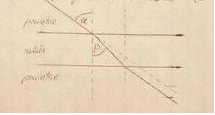
\includegraphics{plytka}
\begin{equation}
h = \frac{d}{n}
\end{equation}
\section{Budowa mikroskopu - jak biegnie promień. Od czego zależy powiększenie obrazu widzianego w mikroskopie?}
Mikroskop optyczny służy do generowania powiększonego obrazu badanego przedmiotu przy wykorzystaniu specjalnego układu optycznego składającego się zwykle z kilku lub kilkanastu soczewek.
Powiększenie mikroskopu, czyli stosunek rozmiaru obrazu do rozmiaru przedmiotu, zależy od iloczynu:
\begin{enumerate}
\item powiększenia obiektywu $p_1$
\item powiększenia okularu $p_2$
\item powiększenia nasadki okularowej ja bym to wywalił xD

powiększenie mikroskopu $p = p_1p_2 = ]$
\end{enumerate}
Aby w mikroskopie powstał ostry obraz, obraz wytworzony przez obiektyw musi znaleźć się prawie w ognisku okularu.\\
{\color{red}NIE MA JAK BIEGNIE PROMIEŃ W MIKROSKOPIE}
\end{document}